\section{Zielsetzung}
Im Versuch wird die Reichweite von Alphastrahlung in Luft ermittelt, sowie der statistische Zerfall analysiert.

\section{Theorie}
Die Entstehung von $\alpha$-Strahlung ist quantenmechanisch erklärbar. Die Kernkräfte und die Abstoßungskräfte der Protonen bilden einen unendlich
hohen Potentialwall. Klassisch ist eine Überwindung dessen nicht erklärbar. Quantenmechanisch besteht jedoch eine Tunnelwahrscheinlichkeit, die
das Überwinden des unendlich hohen Potentialwalls und somit die Entstehung von $\alpha$-Strahlung erklärt.
Beim Durchlaufen von Materie verliert $\alpha$-Strahlung ihre Energie. Dies ist durch drei verschiedene Prozesse zu erklären.
Zum einen durch die sogenannte Rutherford-Streuung, wobei es zu elastischen Stößen zwischen den $\alpha$-Teilchen und den Materieteilchen
kommt, welche für den Energieverlust und somit für den Versuch jedoch nur eine untergeordnete Rolle spielt.
Des weiteren ist ein Energieverlust durch Ionisationsprozesse und Anregung oder Dissoziation von Molekülen zu erklären.
Zu erwähnen ist, dass der Energieverlust der $\alpha$-Strahlung bei kleineren Geschwindigkeiten größer wird, was durch die längere
Zeit zu erklären ist, die die Teilchen zur Wechselwirkung miteinander haben. Außerdem ist der Energieverlust abhängig von der Energie der
$\alpha$-Teilchen selbst, sowie der Dichte des Materials mit dem die Strahlung wechselwirkt.
Die Bethe-Bloch-Gleichung beschreibt den Energieverlust von Teilchen, die eine hinreichend große Anfangsenergie besitzen. Sie verliert ihre
Gültigkeit für $\alpha$-Teilchen mit geringer Energie, weil dann Ladungsaustauschprozesse stattfinden.
\FloatBarrier
\begin{align*}
  - ~\frac{dE_\alpha}{dx} = \frac{z^2~e^4}{4\pi\epsilon_0 m_e}~\frac{n ~ Z}{v^2}~ln\left(\frac{2 m_e v^2}{I}\right) .
\end{align*}
\FloatBarrier
In der Bethe-Bloch-Gleichung beschreibt $z$ die Ladung, $v$ die Geschwindigkeit der $\alpha$-Strahlung, $n$ die Teilchendichte, $Z$ steht für die
Ordnungszahl und $I$ für die Ionisationsenergie des Targetgases.
Die Reichweite von $\alpha$-Strahlung lässt sich dann mittels Integration berechnen:
\FloatBarrier
\begin{align*}
  \int_{0}^{E_{\alpha}} \frac{dE_\alpha}{-dE_\alpha ~ / dx}
\end{align*}
\FloatBarrier
Die mittlere Reichweite $R_m$ von Teilchen mit niedrigerer Energie, bei denen es vermehrt zu Ladungsaustauschprozessen kommt, kann mittels
empirischer gewonnener Kurven bestimmt werden.
Gleichung \ref{eq3} beschreibt die mittlere Reichweite für $\alpha$-Teilchen, die eine Energie unter $\SI{2,5}{\mega \eV}$ besitzen.
Die mittlere Reichweite beschreibt die Distanz, in der noch die Hälfte aller emittierten $\alpha$-Teilchen ankommen.
\FloatBarrier
\begin{align*}
  \label{eq3}
  R_m = 3,1 \cdot E_{\alpha}^{3/2}
\end{align*}
\FloatBarrier
Da die Reichweite von $\alpha$-Strahlung in Gasen druckabhängig ist, gilt zur Ermittlung der Reichweite folgender Zusammenhang:
\begin{align*}
  x = x_0 \frac{p}{p_0}
\end{align*}
Hierbei beschreibt $x_0$ den fixen Abstand zwischen Detektor und Quelle, und $p_0$ den Normaldruck von $\SI{1013}{\bar}$.

\section{Durchführung}
Zur Durchführung des Versuchs wird eine $\alpha$-Strahlungsquelle, ein Detektor, eine Vakuumpumpe zur Evakuierung des Glaszylinders, in dem
sich Quelle und Detektor befinden, ein Vorverstärker, ein Vielkanalanalysator, sowie ein PC, der die vom Detektor gemessenen und vom
Vielkanalanalysator analysierten, Daten aufnimmt, benötigt. Der Versuchsaufbau ist in Abbildung \ref{abb1} zu sehen.
Der Abstand der Quelle ist variabel einzustellen und an einer Skala, die außen auf dem Glaszylinder aufgezeichnet ist, abzulesen.
Der Detektor ist ein Halbleiter-Sperrschichtzähler, welcher den Vorteil besitzt, dass er dazu in der Lage ist Strahlung mit niedrigerer Energie
zu detektieren. Dies geschieht, indem einfallende Ionen in der Sperrschicht des Halbleiters ein Elektron-Loch-Paar erzeugen, welches zu
einem Strompuls im Halbleiter führen, welcher gemessen werden kann. Die erzeugten Pulse werden von dem Vorverstärker verstärkt, vom
Vielkanalanalysator analysiert und an das PC-Programm "Multichannel Analyzer" weitergegeben. Im Programm werden die Pulshöhen, die der Energie
der $\alpha$-Strahlung entsprechen, als Histogramm dargestellt.
\FloatBarrier
\begin{figure}
  \centering
  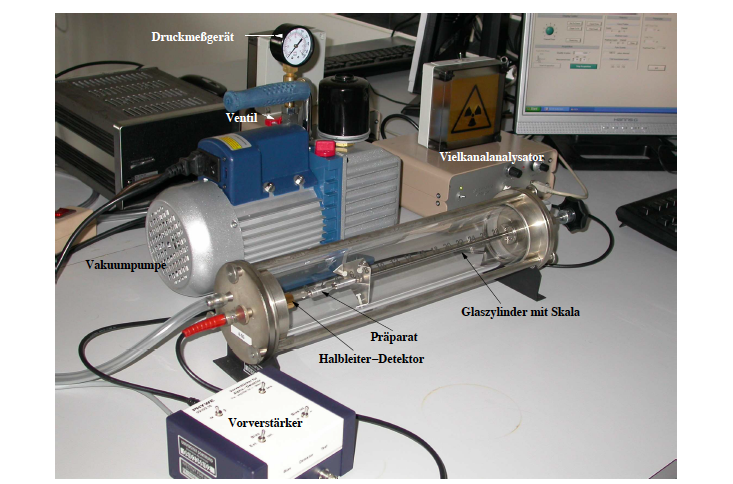
\includegraphics[scale=0.6]{Aufbau.PNG}
  \caption{Versuchsaufbau \cite{Q1}.}
  \label{abb1}
\end{figure}
\FloatBarrier
\noindent Im ersten Teil des Versuchs muss zu Beginn der Glaszylinder evakuiert werden. Die Messdauer eines jeden Schrittes beträgt zwei Minuten.
Nach zwei Minuten Messdauer werden dann die gemessenen Counts insgesamt, die Counts, die sich um das Maximum herum befinden, sowie die
Lage des Maximums notiert. Es wird davon ausgegangen, dass die detektierte $\alpha$-Strahlung bei $\SI{0}{\milli \bar}$ eine Energie
von $\SI{4}{\mega \eV}$ besitzt. Aus der Anzahl der Counts im Maximum lässt sich mittels Dreisatz die Energie für höhere Drücke
berechnen. Der Druck wird schrittweise um $\SI{50}{\milli \bar}$ erhöht und die drei oben erwähnten Werte werden jeweils nach zwei Minuten Messzeit
notiert. Der Druck kann bis $\SI{1000}{\milli \bar}$ erhöht werden. Es ist daher wichtig, dass im Vorfeld klargestellt wurde, dass die Apparatur
so eingestellt ist, dass bei diesem maximalen Druck nur noch sehr wenige bis gar keine Counts insegsamt mehr detektiert werden.
Am Versuchstag wurde diese Überprüfung bereits im Vorfeld, jedoch nicht von uns durchgeführt.
Die oben beschriebene Messung wird einmal bei einem Abstand zwischen Quelle und Detektor von $\SI{2}{\cm}$ und ein weiteres Mal für einen Abstand
von $\SI{2,5}{\cm}$ durchgeführt.

\noindent Zur Ermittlung des statistischen Zerfalls werden im evakuierten Glaszylinder für 100 Messungen bei einem Abstand von $\SI{2}{\cm}$
über $\SI{10}{\second}$ die Gesamtcounts gemessen und notiert. Die Zerfallsraten werden sodann in einem Histogramm aufgetragen und es werden
Mittelwert und Varianz der Zählraten bestimmt. Anschließend werden die Ergebnisse mit der Poisson- und der Gaußverteilung verglichen.
